\subsection{Divisão e conquista}

    Divisão e Conquista é uma técnica que pode ser dividida em três 
    partes fundamentais: dividir um problema maior recursivamente em 
    problemas menores(\textbf{Dividir}), resolver todos os 
    sub-problemas (\textbf{Conquistar}) e, por fim, a solução do problema inicial 
    é dada através da combinação dos resultados de todos os problemas 
    menores computados(\textbf{Combine}). 

    Problemas que usam divisão e conquista são característiscos em possuir um princípio 
    chamado \textbf{Overlapping subproblems}, ou seja, o problema pode ser divido em 
    subproblemas, que são reutilizados várias vezes e que não geram novos subproblemas.
    
    Exemplos de problemas conhecidos que usam desta estratégia são o problema de 
    ordenação interna(usando quicksort ou mergesort) e o problema dos pares de pontos próximos.

\subsubsection{Pares de pontos próximos}

    Dado um conjunto de N pontos em um espaço, é preciso encontrar os dois pontos do conjunto que possuem a 
    menor distância um do outro. Este problema possui mais de uma implementação, porém 
    uma das mais eficientes é utilizando divisão e conquista.

    \begin{figure}[ht]
        \centering
        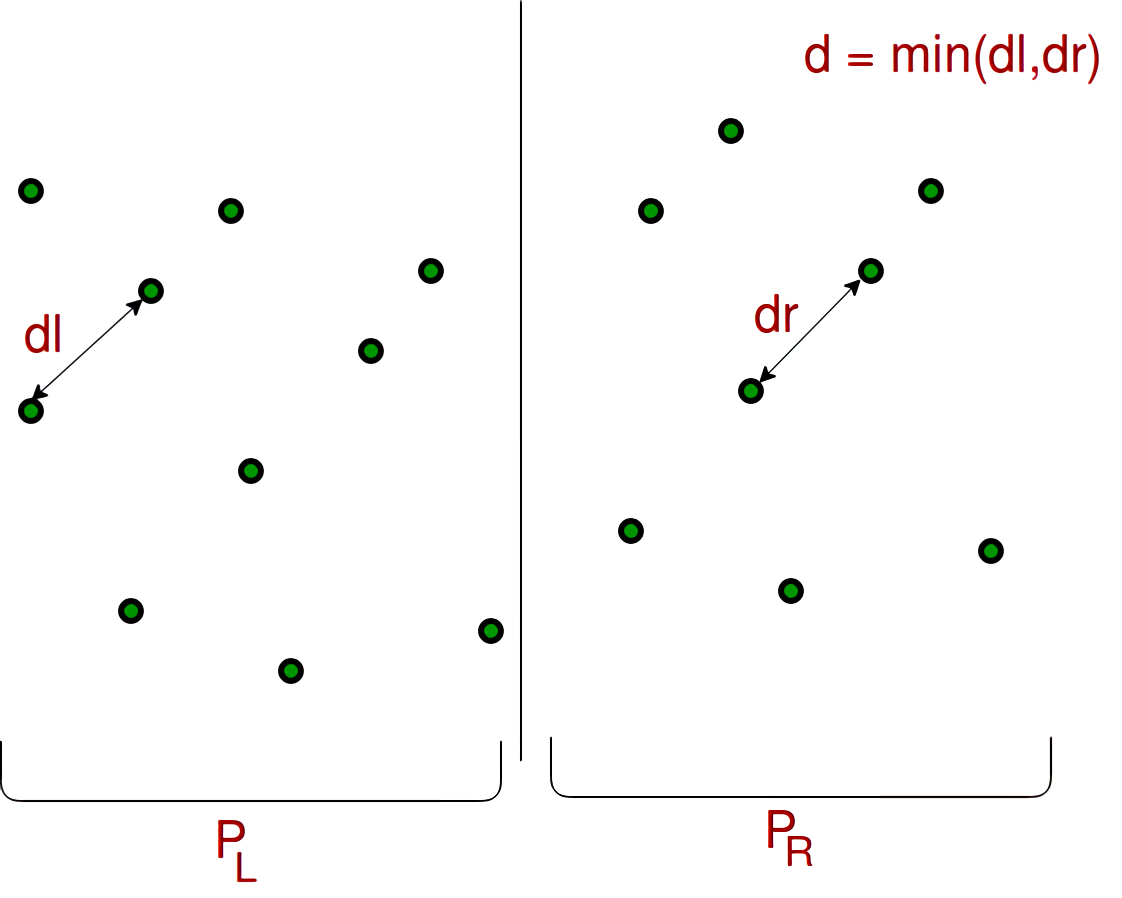
\includegraphics[width=.5\textwidth]{divide-and-conquer.png}
        \caption{Uma representação visual da separação dos pontos}
        \label{fig:divide-and-conquer}
    \end{figure}

    Supondo que a entrada para o problema é um conjunto de pontos com o eixo y já ordenado,
    encontramos o ponto do meio, separamos o conjunto ao meio, e então recursivamente descobrimos
    as menores distâncias entre os conjuntos separados, para então achar a solução geral.

    \newpage 

    \begin{algorithm}
        \caption{Closest pair of points} 
        \begin{algorithmic}[1]
        \Procedure{Divide-and-conquer}{P,Q}
        \If{$n \geq 3$}
        \State {$\textbf{bruteForce(P,n)}$}
        \EndIf
        \State {$midPoint$ $\gets$ $P[\frac{n}{2}]$}
        \State {$P_l$ $\gets$ $P[1...\frac{n}{2}-1]$}
        \State {$Q_l$ $\gets$ $P[1...\frac{n}{2}-1]$}
        \State {$P_r$ $\gets$ $P[\frac{n}{2}...n]$}
        \State {$Q_r$ $\gets$ $P[\frac{n}{2}...n]$}
        \State {$d_l$ $\gets$ $DIVIDE-AND-CONQUER(P_l,Q_l)$}
        \State {$d_r$ $\gets$ $DIVIDE-AND-CONQUER(P_r,Q_r)$}
        \State {$d$ $\gets$ $min(d_l,d_r)$}
        \State {$strip_p$ $\gets$ $[]$}
        \State {$strip_q$ $\gets$ $[]$}
        \State {$lr$ $\gets$ $P_l + P_r$}
        \For {$\text{i \textbf{to} n}$}
        \If{$abs(lr[i].x - midPoint.x) < d$}
        \State{$stripP.append(lr[i])$}
        \EndIf
        \If{$abs(Q[i].x - midPoint.x) < d$}
        \State{$stripQ.append(Q[i])$}
        \EndIf
        \EndFor
        \State {$sort(stripP,key = y)$}
        \State {$min_p$ $\gets$ $min(d, stripClosest(striP), \mid stripP \mid , d )$}
        \State {$min_q$ $\gets$ $min(d, stripClosest(striQ), \mid stripQ \mid , d )$}
        \State {$\textbf{return } $ $min(min_p,min_q)$}
        \EndProcedure
        \end{algorithmic}
      \end{algorithm}

      \subsubsection{Divisão e Conquista Vs Backtracking}

      \begin{itemize}
          \item Devido à maneira como ambos são conceitualizados, ambos possuem a 
          natureza de serem recursivos.
          \item Em divisão e conquista, precisamos analisar a entrada inteira do usuário 
          para resolver o problema, enquanto que Backtracking pode ou não analisar a todas 
          as possibilidades dentro da entrada do usuário
      \end{itemize}

      \subsubsection{Divisão e Conquista Vs Branch and Bound}

      \begin{itemize}
          \item Enquanto divisão e conquista divide a entrada do usuário(Ex: divide o vetor de 
          números para ordená-los) para resolver os sub-problemas e então resolver a combinação
          desses problemas, a outra estratégia divide o espaço da solução para o problema.
          \item Tanto Branch and Bound e Divide and Conquer são estratégias que partem dos 
          mesmos princípios: ambas querem dividir o problema em partes menores para resolver 
          o problema todo.
      \end{itemize}

    \nocite{divide-and-conquer}
    \nocite{closest-pair-of-points}
\newpage